\documentclass[11pt,a4paper]{article}

% ── Packages ──────────────────────────────────────────────────────
\usepackage[utf8]{inputenc}
\usepackage[T1]{fontenc}
\usepackage{lmodern}
\usepackage[margin=2.5cm]{geometry}
\usepackage{graphicx}
\usepackage{xcolor}
\usepackage{booktabs}
\usepackage{amsmath,amssymb}
\usepackage{hyperref}
\usepackage{natbib}

\hypersetup{
  colorlinks=true,
  linkcolor=blue!50!black,
  citecolor=blue!50!black,
  urlcolor=blue!60!black
}

\newcommand{\att}{ATT}
\newcommand{\mpol}{MaxPressure}
\newcommand{\repo}{\texttt{LibSignalFork}}

\title{%
  Realism-Composed Benchmarking for Traffic Signal Control:\\
  When Classical Controllers Do Not Fail Under Realistic Simulation
}
\author{%
  Anonymous Authors\\
  \small\textit{[names / affiliations TBD --- see \texttt{paper/notes/OPEN\_QUESTIONS.md}]}
}
\date{Draft --- \today}

\begin{document}
\maketitle

\begin{abstract}
Reinforcement learning (RL) for traffic signal control (TSC) is routinely evaluated on homogeneous, fully observed microsimulations with a single fixed demand ``movie.''
Under those conditions, learned policies often appear to dominate classical network controllers such as max-pressure.
We argue that this comparison conflates \emph{algorithmic advantage} with \emph{simulation idealism}.
Building on LibSignal~\citep{mei2023libsignal}, we introduce a \textbf{realism-composed} benchmarking protocol with five independently toggled realism axes---heterogeneous fleets, slow-start discharge, actuated pedestrian crossing proxies, connected-vehicle penetration, and Gaussian count noise---plus a hub-centric origin--destination (OD) demand set with held-out evaluation.
Across corrected \texttt{sumo4x4} grids and an Ingolstadt $1{\times}21$ arterial, we find that (i)~rankings are fragile under topology and realism; (ii)~effect sizes between RL and \mpol are often small relative to the ATT uplift induced by realism itself; and (iii)~under compound plant+sensor stress, \mpol remains a strong anchor while several RL agents degrade, contrary to narratives that classical methods ``fail'' in realistic environments.
We additionally analyze trip-level travel-time distributions, idle-share metrics, and a ghost-physics ceiling baseline, and outline ongoing work on actor--critic agents and LLMLight-style controllers.
\end{abstract}

\tableofcontents
\newpage

% =============================================================================
\section{Introduction}
\label{sec:intro}

Traffic signal control (TSC) sits at the intersection of transportation engineering and multi-agent learning.
Classical methods range from fixed-time Webster plans~\citep{webster1958} to theoretically grounded network policies such as max-pressure~\citep{varaiya2013maxpressure}.
Over the last decade, deep RL methods---IntelliLight~\citep{wei2018intellilight}, PressLight~\citep{wei2019presslight}, CoLight~\citep{wei2019colight}, MPLight~\citep{chen2020mplight}, and others---have reported large gains over these baselines in microsimulation.
Open libraries such as LibSignal~\citep{mei2023libsignal} and RESCO~\citep{ault2021resco} make such comparisons reproducible across SUMO~\citep{lopez2018sumo} and CityFlow~\citep{zhang2019cityflow}.

Yet a growing body of work argues that RL-TSC has not closed the sim-to-real gap~\citep{chen2022realdeal,wei2019survey,yau2017survey}.
Benchmarks often assume homogeneous vehicles, perfect detectors, no pedestrians, and a single repeating demand file.
In that setting, learned policies can memorize the traffic movie rather than control under uncertainty.
Moreover, RL papers frequently motivate their methods by stating that max-pressure is greedy, assumes unlimited downstream capacity, or fails under complex realistic networks~\citep{wei2019presslight,wei2019colight}---claims that are theoretically nuanced and empirically under-tested once the \emph{simulator} itself becomes realistic.

\paragraph{Central claim.}
When we \emph{introduce realism into the simulation} in a controlled, compositional way, we do \textbf{not} observe a systematic collapse of max-pressure relative to popular RL controllers.
Instead, rankings reshuffle with topology and realism profile; absolute effect sizes are often small; and compound realism can hurt RL as much as---or more than---classical baselines.

\paragraph{Contributions.}
\begin{enumerate}
  \item A \textbf{realism-axis taxonomy} (plant vs.\ sensor) implemented in SUMO/LibSignal, with single-axis ablations and a composed \texttt{realism\_full} profile.
  \item A \textbf{demand-realism} protocol: hub-centric OD generation, train/hold splits, and held-out mean ATT (\texttt{HELDOUT\_MEAN}).
  \item Empirical evidence on \texttt{sumo4x4} (reproduction + realism) and ongoing Ingolstadt~\texttt{sumo1x21} arterial experiments showing topology-dependent rankings and fragile leaderboards.
  \item Metric critique: trip-level distributions, idle share, and discussion of an effectiveness estimator based on idle/travel time.
  \item A ghost-physics baseline that removes vehicle--vehicle interaction while retaining signal obedience, as an unrealistic performance ceiling.
\end{enumerate}

\paragraph{Status of this draft.}
Numbers in Tables~\ref{tab:homo4x4}--\ref{tab:odh4x4} are backed by logs under \texttt{data/output\_data/} and notebooks under \texttt{result\_analysis/} (read-only; not modified for this draft).
Ingolstadt OD-hub L1/L2 sync is still incomplete locally; actor--critic and LLMLight results are planned (Sec.~\ref{sec:future}).

% =============================================================================
\section{Related Work}
\label{sec:related}

\subsection{Classical and learning-based TSC}
Max-pressure~\citep{varaiya2013maxpressure} selects the phase that maximizes local pressure (upstream minus downstream occupancy) and is throughput-optimal under idealized queueing assumptions.
PressLight~\citep{wei2019presslight} connects RL rewards to pressure minimization, arguing that greedy MP can be locally suboptimal when physical queues expand.
CoLight~\citep{wei2019colight} uses graph attention for network-level cooperation and also positions MP as limited by capacity assumptions.
Surveys catalog reward/state design choices and coordination challenges~\citep{wei2019survey,yau2017survey,noaeen2021recent}.
Empirical corridor studies of cyclic MP variants in realistic demand settings report that carefully engineered MP can remain competitive with deployed actuated control~\citep{islam2022mprealistic}---a transportation-side counterpoint to ``MP fails in reality'' narratives in the ML literature.

\subsection{Benchmarks and scenarios}
LibSignal~\citep{mei2023libsignal} unifies agents and metrics across simulators and reports Grid$4{\times}4$ SUMO tables that we reproduce as a gate.
RESCO~\citep{ault2021resco} emphasizes real-city networks (Cologne, Ingolstadt) and shows that which RL algorithm wins depends on the scenario---already a hint that rankings are topology-sensitive.
CityFlow~\citep{zhang2019cityflow} accelerates large-scale MARL experiments but can encourage idealized sensing and demand unless realism is added explicitly.

\subsection{Sim-to-real barriers}
Chen et al.~\citep{chen2022realdeal} organize deployment barriers into detection uncertainty, communication reliability, compliance/interpretability, and heterogeneous road users.
Tan et al.~\citep{tan2020robust} inject Gaussian noise into queue features during training; Rodrigues and Azevedo~\citep{rodrigues2019towards} study demand surges, incidents, and sensor failures.
Our axes operationalize several of these challenges as \emph{composible toggles} with ground-truth ATT preserved under observation corruption.

\subsection{Evaluation fragility in deep RL}
Outside TSC, Henderson et al.~\citep{henderson2018matters} and Colas et al.~\citep{colas2018seeds} show that seed variance and small effect sizes inflate apparent wins; Agarwal et al.~\citep{agarwal2021rliable} advocate distributional reporting.
We bring this lens to TSC: mean ATT over one seed and one demand movie is a thin ranking signal when realism can move ATT by tens of seconds.

\subsection{Emerging LLM controllers}
LLMLight~\citep{lai2024llmlight} frames TSC as language-mediated reasoning with strong claims of generalization and interpretability.
We treat it as a future comparator under the same realism protocol, not as a settled SOTA claim.

% =============================================================================
\section{Problem Setting and Protocol}
\label{sec:protocol}

\subsection{Environment}
We use LibSignal~\citep{mei2023libsignal} with SUMO~\citep{lopez2018sumo} via \texttt{libsumo}.
Primary networks:
\begin{itemize}
  \item \textbf{\texttt{sumo4x4}}: corrected Grid$4{\times}4$ after a TLS audit (pre-fix network had invalid NEMA \texttt{s} placements; reproduction matched LibSignal Table~8 but was invalid for realism work---see \texttt{docs/SIGNAL\_CONTROL\_THEORY.md}).
  \item \textbf{\texttt{sumo1x21}}: Ingolstadt arterial corridor (21 signalized intersections), drawn from RESCO/InTAS-style packs~\citep{ault2021resco}.
\end{itemize}
Unless noted, seed $=42$, action interval $10$\,s, episode horizon $3600$\,s for movie-style runs and $1800$\,s for OD-hub runs.

\subsection{Agents}
Classical: FixedTime, MaxPressure.
RL (current): DQN, PressLight, CoLight (LibSignal defaults).
Planned: IPPO/PPO~\citep{schulman2017ppo}, MADDPG~\citep{lowe2017maddpg}, LLMLight~\citep{lai2024llmlight}.

\subsection{Primary metric}
Average travel time (\att) over completed trips (ground-truth physics).
Under partial observability, queue/reward logs are \emph{observed}; ATT is never corrupted.
For OD-hub: \texttt{HELDOUT\_MEAN} over three held-out route files.

% =============================================================================
\section{Realism Axes}
\label{sec:axes}

We separate \textbf{plant} axes (change physics / delay structure) from \textbf{sensor} axes (corrupt what the controller sees).
Defaults are exact no-ops so the homogeneous LibSignal baseline is recoverable.

\subsection{Plant axes}
\begin{description}
  \item[A1 Heterogeneous fleet.]
    Mix of passenger cars and trucks (default $80\%/20\%$) with distinct lengths and dynamics (\texttt{grid4x4\_hetero.rou.xml}).
  \item[A2 Slow-start discharge.]
    Reduced acceleration / increased headway ($\tau$) via custom \texttt{vType}s, modeling sluggish queue discharge after green.
  \item[A3 Crossing proxy.]
    Actuated concurrent pedestrian walk without explicit \texttt{<person>} agents: with probability $p{=}0.12$ on through-green entry, hold green for $T\sim\mathrm{Unif}(7,10)$\,s and halt mapped through lanes (see repo doc \texttt{docs/CROSSING\_PROXY.md}; implementation in \texttt{world/world\_sumo.py}).
\end{description}

\subsection{Sensor axes}
\begin{description}
  \item[A4 Penetration.]
    Each vehicle is visible for its entire trip w.p.\ $p$ (default $0.8$); lane counts built from the visible subset~\citep{chen2022realdeal}.
  \item[A5 Count noise.]
    Per-lane additive Gaussian noise $\mathcal{N}(0,\sigma^2)$ with $\sigma{=}2$, clamped $\ge 0$, resampled each step~\citep{tan2020robust}.
\end{description}

\subsection{Composition: \texttt{realism\_full}}
All five axes on simultaneously (\texttt{configs/tsc/realism\_full\_world.yml}).
Agents train and evaluate on the same profile (no train-on-homo / test-on-realism transfer unless stated).
Interactions need not be additive: compound ATT uplift can exceed the sum of single-axis deltas.

\subsection{Demand realism (OD-hub)}
Separate from plant/sensor axes, we generate hub-centric OD demand with fringe/within origins, shoulder+peak timeline, and stochastic train/hold files (\texttt{extras/gen\_od\_hub\_demand\_grid4x4.py}; validation in \texttt{result\_analysis/od\_hub\_demand\_distribution.md}).
\begin{itemize}
  \item \textbf{L1:} OD-hub only (homo plant, full obs).
  \item \textbf{L2:} OD-hub + \texttt{realism\_full}.
\end{itemize}
This tests generalization beyond a single movie~\citep{ault2021resco}.

\subsection{Ghost-physics ceiling}
\texttt{physics\_mode: ghost} makes vehicles ignore each other while still obeying reds---an unrealistic lower bound on conflict delay (\texttt{docs/TRAINING\_GUIDE.md}).
We treat ghost FixedTime/MaxPressure as a \emph{ceiling}, not a peer baseline.

% =============================================================================
\section{Additional Metrics and Ranking Questions}
\label{sec:metrics}

Mean ATT is the community default, but it compresses a right-skewed trip distribution.
On homo \texttt{sumo4x4} we export per-trip travel time, waiting fraction
\begin{equation}
  w_i = \frac{T^{\mathrm{idle}}_i}{T_i},
\end{equation}
and discuss schedule efficiency $T^{\mathrm{ff}}_i / T_i$.

\paragraph{Effectiveness estimator (under evaluation).}
One candidate ranking measure is the mean idle share
\begin{equation}
  E = \frac{1}{N}\sum_{i=1}^{N} \frac{T^{\mathrm{idle}}_i}{T_i},
\end{equation}
i.e., fraction of each trip spent essentially stopped.
On the default homo grid, $E$ separates FixedTime from MP/DQN more sharply than ATT alone, but does not reorder them (Sec.~\ref{sec:results4x4}).
Whether $E$ is worth promoting as a primary metric under OD-hub / arterial settings remains an open question (see clarifications).

\paragraph{Effect size vs.\ rank.}
We emphasize absolute $\Delta$\att (seconds) and rank changes across profiles, not only ``method~$A$ beats method~$B$.''
When realism itself adds $+50$--$100$\,s of ATT, a $+3$\,s RL win on the toy homo grid is not decision-relevant.

% =============================================================================
\section{Experiments on Grid $4{\times}4$}
\label{sec:results4x4}

\subsection{Reproduction gate and TLS correction}
On the \emph{pre-fix} network we approximately matched LibSignal Table~8 (SUMO Grid$4{\times}4$).
After correcting NEMA phases, homo baselines shift (Table~\ref{tab:homo4x4}): MaxPressure $173.3$\,s, FixedTime $219.1$\,s.
All realism results use the corrected network.

\begin{table}[t]
\centering
\caption{Homo \texttt{sumo4x4}, seed~42, corrected TLS. RL: best/final test ATT over 200 episodes; baselines: BRF final.}
\label{tab:homo4x4}
\begin{tabular}{lrr}
\toprule
Method & Best/Final ATT (s) & Notes \\
\midrule
DQN        & 167.8 / 167.9 & \\
CoLight    & 168.9 / 173.1 & \\
MaxPressure& 173.3 / 173.3 & BRF \\
PressLight & 171.9 / 174.4 & \\
FixedTime  & 219.1 / 219.1 & BRF \\
\bottomrule
\end{tabular}
\end{table}

\subsection{Single-axis ablations}
Table~\ref{tab:axes4x4} summarizes final ATT under each axis.
Patterns:
\begin{itemize}
  \item Slow-start and hetero add a modest ATT tax ($\sim$10--20\,s) without reversing the MP$\approx$RL band.
  \item Penetration ($p{=}0.8$) mildly hurts everyone; Gaussian $\sigma{=}2$ is harsher and destabilizes CoLight.
  \item Crossing proxy adds $\sim$5--8\,s vs.\ homo for most methods.
\end{itemize}

\begin{table}[t]
\centering
\caption{Single-axis realism on corrected \texttt{sumo4x4} (final ATT, seed~42).}
\label{tab:axes4x4}
\setlength{\tabcolsep}{4pt}
\begin{tabular}{lrrrrr}
\toprule
Method & Homo & Slow & Hetero & Obs $p{=}0.8$ & Noise $\sigma{=}2$ \\
\midrule
DQN         & 167.9 & 185.3 & 184.0 & 183.3 & 231.8 \\
CoLight     & 173.1 & 190.4 & 189.1 & 185.1 & 312.2 \\
MaxPressure & 173.3 & 186.1 & 189.4 & 185.4 & 200.9 \\
PressLight  & 174.4 & 191.0 & 189.3 & 185.8 & 201.9 \\
FixedTime   & 219.1 & 243.7 & 240.5 & 219.7 & 219.7 \\
\bottomrule
\end{tabular}
\end{table}

Crossing-proxy finals (vs.\ homo): DQN $174.4$~($+6.5$), MP $178.4$~($+5.2$), CoLight $179.6$~($+6.5$), PressLight $182.6$~($+8.2$), FixedTime $223.5$~($+4.4$).

\subsection{Compound realism (\texttt{realism\_full})}
Table~\ref{tab:full4x4} is the capstone: all plant+sensor axes on; RL trained on-profile.

\begin{table}[t]
\centering
\caption{\texttt{realism\_full} on \texttt{sumo4x4}. $\Delta$ vs.\ homo and vs.\ MP under the same profile.}
\label{tab:full4x4}
\begin{tabular}{lrrr}
\toprule
Method & Final ATT & $\Delta$ vs.\ homo & $\Delta$ vs.\ MP \\
\midrule
MaxPressure & 237.5 & $+64.3$ & $0$ \\
PressLight  & 248.0 & $+73.6$ & $+10.5$ \\
FixedTime   & 271.0 & $+51.9$ & $+33.5$ \\
DQN         & 282.8 & $+114.9$ & $+45.3$ \\
CoLight     & 494.6 & $+321.5$ & $+257.1$ \\
\bottomrule
\end{tabular}
\end{table}

\textbf{Interpretation.}
Compound stress raises MP by $+64$\,s---larger than any single axis.
Pressure-aligned PressLight stays near MP; vanilla DQN and especially CoLight degrade.
This contradicts the marketing narrative that realism preferentially sinks classical MP while elevating deep RL.

\begin{figure}[t]
\centering
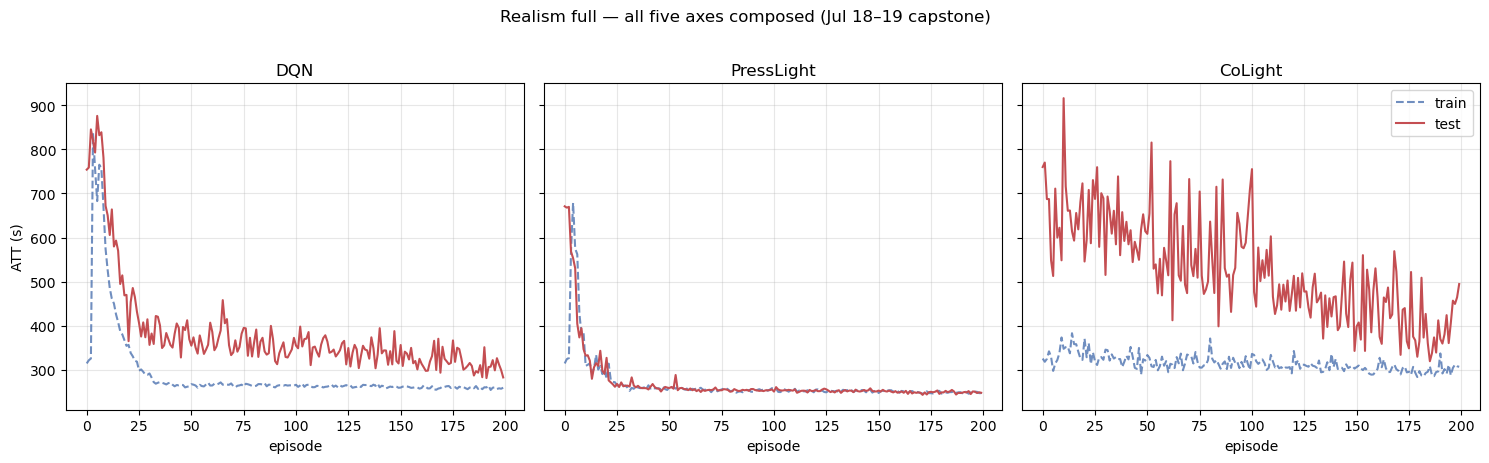
\includegraphics[width=0.95\linewidth]{figures/realism_benchmark_4x4_c30_i6.png}
\caption{Learning curves under \texttt{realism\_full} (train dashed, test solid). Source: \texttt{result\_analysis/realism\_benchmark\_4x4.ipynb}.}
\label{fig:fullcurves}
\end{figure}

\subsection{OD-hub L1 / L2}
Held-out means (Table~\ref{tab:odh4x4}): under demand-only L1, DQN/CoLight/MP are tightly clustered ($\sim$157\,s).
Under L2 (demand + \texttt{realism\_full}), MP ($186.9$) and PressLight ($190.9$) remain anchors; DQN and CoLight inflate sharply.

\begin{table}[t]
\centering
\caption{OD-hub held-out ATT on \texttt{sumo4x4} (seed~42).}
\label{tab:odh4x4}
\begin{tabular}{lrrr}
\toprule
Method & L1 held-out & L2 held-out & $\Delta$ (L2$-$L1) \\
\midrule
MaxPressure & 157.2 & 186.9 & $+29.7$ \\
PressLight  & 163.4 & 190.9 & $+27.5$ \\
FixedTime   & 186.6 & 192.2 & $+5.6$ \\
DQN         & 156.9 & 245.3 & $+88.4$ \\
CoLight     & 157.5 & 436.4 & $+278.9$ \\
\bottomrule
\end{tabular}
\end{table}

\subsection{Trip-level distributions}
On homo 4$\times$4, travel times are right-skewed; median rankings match mean rankings (DQN $\approx$ MP $\ll$ FixedTime).
Median waiting fraction $\approx 0.05$ (MP/DQN) vs.\ $\approx 0.22$ (FixedTime)---mechanism insight without leaderboard reversal (Fig.~\ref{fig:tripdist}).

\begin{figure}[t]
\centering
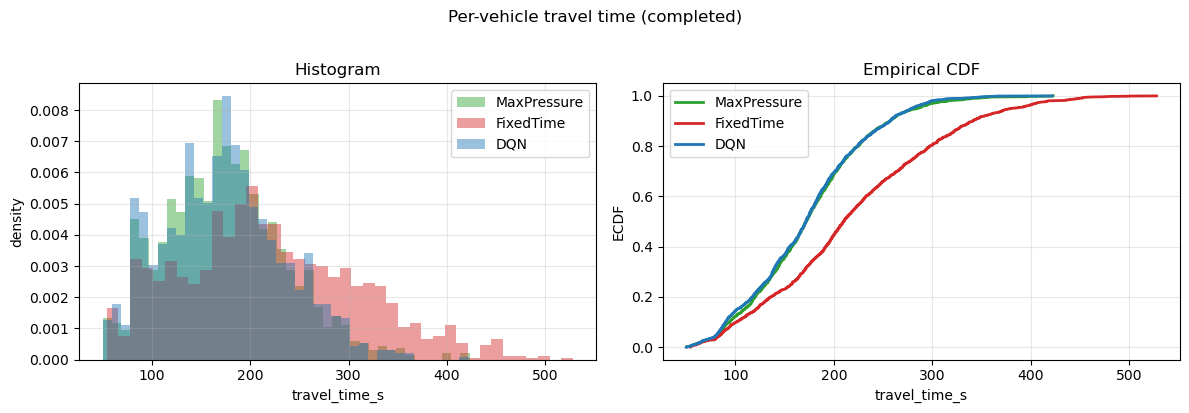
\includegraphics[width=0.85\linewidth]{figures/improved_metrics_c05_i0.png}
\caption{Per-trip travel-time distributions (homo 4$\times$4). Source: \texttt{improved\_metrics.ipynb}.}
\label{fig:tripdist}
\end{figure}

% =============================================================================
\section{Experiments on Ingolstadt $1{\times}21$}
\label{sec:ingo}

The arterial changes the coordination problem: long chains, afternoon-peak demand, and weaker ``local grid pressure'' structure.

\paragraph{Homo baselines (early-stop protocol).}
Primary ATT: PressLight $203.2$, MaxPressure $209.1$, DQN $236.5$, FixedTime $248.9$, CoLight $272.5$ (seed~42).
Fixed-200 episodes reshuffle slightly (PressLight $213.0$, MP $217.8$, DQN $224.4$), illustrating that even budget/early-stop choices move ranks inside a tight band.

\paragraph{Topology-dependent ranking.}
Relative to 4$\times$4---where multiple RL agents sit at or below MP---the arterial favors PressLight~$\approx$~MP, with CoLight often lagging.
Absolute ATT is not comparable across networks; we compare ranks and who beats MP.

\paragraph{Partial status.}
Several single-axis and OD-hub L1/L2 loggers still need sync from compute nodes (\texttt{needs update} in \texttt{ingolstadt21.ipynb}).
Draft claim reserved for the full table: sensor axes (esp.\ penetration) are more destructive on the corridor than on the grid; classical MP can also fail under severe obs corruption---realism hurts \emph{everyone}, not selectively classical methods.

\begin{figure}[t]
\centering
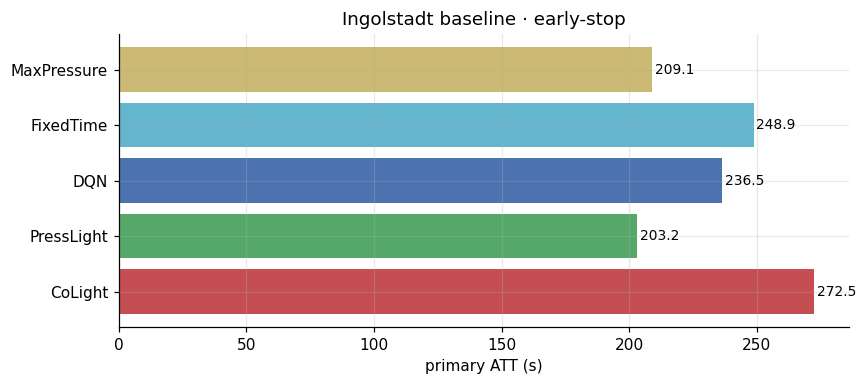
\includegraphics[width=0.95\linewidth]{figures/ingolstadt21_c05_i0.png}
\caption{Ingolstadt homo early-stop learning curves (excerpt). Source: \texttt{ingolstadt21.ipynb}.}
\label{fig:ingo}
\end{figure}

% =============================================================================
\section{Discussion}
\label{sec:discussion}

\paragraph{Does max-pressure ``fail'' under realism?}
In our composed profiles, MP remains competitive or best among the tested set.
RL wins on idealized grids are often a few seconds; realism shifts are tens to hundreds of seconds.
When RL beats MP, the margin is frequently smaller than the uncertainty induced by seed, early-stopping, or axis toggles---consistent with broader RL evaluation critiques~\citep{henderson2018matters,agarwal2021rliable}.

\paragraph{Why do some papers claim otherwise?}
Common arguments: MP is greedy; unlimited downstream capacity; no learning of coordination~\citep{wei2019presslight,wei2019colight}.
Those statements concern \emph{model assumptions}, not empirical failure under every realistic plant.
Our results suggest that once the simulator includes the same detection/fleet/pedestrian frictions that motivate RL papers, the classical baseline often degrades more gracefully than graph RL trained under those frictions.

\paragraph{Is ranking even the right product?}
If changing network or realism profile reorders methods, publishing a single ``SOTA on LibSignal Table~8'' is misleading.
We recommend reporting: (i)~axis-wise ATT, (ii)~compound profile, (iii)~held-out demand, (iv)~effect sizes vs.\ MP, (v)~trip distribution summaries.

\paragraph{Action interval and ``seconds that matter.''}
Many RL-TSC stacks decide every $5$--$10$ simulation seconds.
Claimed wins of $2$--$3$ seconds of ATT should be interpreted relative to that decision granularity and to measurement noise---another reason to prefer effect-size reporting over ordinal ranks.

% =============================================================================
\section{Limitations}
\label{sec:limitations}

\begin{itemize}
  \item Mostly seed~$42$; multi-seed statistical tests are incomplete~\citep{colas2018seeds}.
  \item Crossing proxy is not full multimodal pedestrian simulation.
  \item OD-hub is synthetic hub gravity, not city LODES calibration.
  \item Ingolstadt OD-hub and some axes await logger sync.
  \item Actor--critic and LLMLight not yet under the same protocol.
  \item Ghost physics is a ceiling, not a fair peer.
\end{itemize}

% =============================================================================
\section{Future Work}
\label{sec:future}

\begin{enumerate}
  \item Finish Ingolstadt axis + OD-hub tables; multi-seed sweeps.
  \item Add IPPO / MADDPG under identical realism profiles.
  \item Port LLMLight~\citep{lai2024llmlight} evaluation under \texttt{realism\_full} and held-out OD.
  \item Decide whether idle-share effectiveness $E$ becomes a secondary official metric.
  \item Optional: train-on-homo / test-on-realism transfer gaps (true sim-to-real within sim).
\end{enumerate}

% =============================================================================
\section{Conclusion}
\label{sec:conclusion}

We proposed realism-composed benchmarking for TSC: five axes, demand held-outs, and compound profiles on LibSignal/SUMO.
Empirically, introducing realism does not preferentially invalidate max-pressure in favor of RL; rankings are fragile, effect sizes are often small, and compound stress can collapse sophisticated RL agents while classical pressure control remains an anchor.
We advocate reporting realism profiles and effect sizes---not only leaderboard ranks on idealized movies.

\section*{Reproducibility}
Code and configs: this repository (\repo).
Axis docs: \texttt{docs/PARTIAL\_OBSERVABILITY.md}, \texttt{docs/CROSSING\_PROXY.md}, \texttt{docs/REALISM\_FULL.md}, \texttt{docs/OD\_HUB\_DEMAND.md}.
Analysis notebooks (do not edit for paper assets): \texttt{result\_analysis/*.ipynb}.
Figures in \texttt{paper/figures/} were extracted from notebook outputs without modifying the notebooks.

\bibliographystyle{plainnat}
\bibliography{references}

\appendix
\section{Figure inventory}
\label{app:figs}
See \texttt{paper/figures/MANIFEST.json} for the mapping from extracted PNGs to source notebooks/cells.
Key paper figures currently use:
\texttt{realism\_benchmark\_4x4\_c30\_i6.png},
\texttt{improved\_metrics\_c05\_i0.png},
\texttt{ingolstadt21\_c05\_i0.png}.

\section{Repo mapping of claims}
\label{app:claims}
See \texttt{paper/notes/CLAIMS\_MAP.md}.

\end{document}
